\begin{savequote}[8cm]
\textlatin{Neque porro quisquam est qui dolorem ipsum quia dolor sit amet, consectetur, adipisci velit...}

There is no one who loves pain itself, who seeks after it and wants to have it, simply because it is pain...
  \qauthor{--- Cicero's \textit{de Finibus Bonorum et Malorum}}
\end{savequote}

\chapter{\label{ch:5-tki}TKI} 

\minitoc

\section{in ND up}


       Neutrino-nucleus interaction is an overarching term including complicated effects besides the most fundamental neutrino-nucleon interaction. 
       First of all, the nucleons in the nucleus have different initial nuclear states (IS). 
       There is no way to determine their kinematics before its interaction with the neutrino. 
       They can only be estimated from nuclear models, which have no definitive answers and are still hot topics of current research. 
       Moreover, there could be correlation between a pair of nucleons such that the interaction between a neutrino and one nucleon can affect another nucleon significantly as well. Last but not least, after the neutrino-nucleon interaction, the final products are still inside the nucleus. 
       On their way out, it is not uncommon that they interact with the nuclear medium on their way out of the nuclei so that their kinematics are drastically altered. 
       These are the so-called Final State Interactions (FSI). 
       After they leave the nucleus, they can then be detected by our detectors if they possess energy above the detection threshold. 
       Hence, measurements of particle kinematics from the neutrino-nucleus interaction are unavoidably a convolution of all these effects, each approximated by a model. 
    
        \begin{figure}[!htb] 	
            \centering 		
            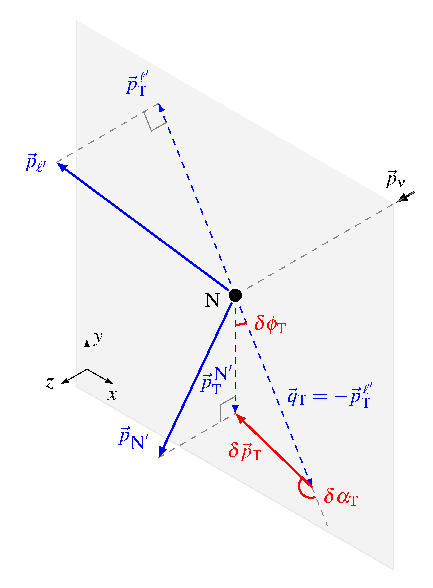
\includegraphics[width=0.35\textwidth]{figures/stki.eps}
            \caption{\label{fig:stki} Schematic illustration of the TKI variables. Diagram taken from Ref.~\cite{Lu:2015tcr}.} 
        \end{figure}
    
       The TKI variables are shown in Fig.~\ref{fig:stki}. They are cleverly constructed such that they are most sensitive to IS and FSI. 
       In the simplest case, there are only two final particles after the neutrino-nucleon interaction, a muon and a proton. 
       If the initial momentum of the struck nucleon has no component transverse to the neutrino's incoming direction, the products, i.e. the muon and the proton, should not have a net transverse component either, unless the struck nucleon has a non-zero initial transverse component or the final particles have undergone FSI.
       Suppose there is no FSI, the net transverse component, $\dpt$, corresponds exactly to the magnitude of the transverse component of the struck nucleon, and the angle, $\dat$, represents the direction of the initial nucleon motion projected on the transverse plane. 
       Assuming the nucleons are moving isotropically, the $\dat$ distribution should be flat. 
       All current nuclear models do not have a preferential direction for initial nuclear motion, so it is only natural to assume the nucleons move in random directions. 
       Thus, the deviation from flatness for $\dat$ can only be due to FSI, thereby making it an excellent probe for FSI. 
       As for $\dpt$, it reflects the magnitude of the initial nucleon momentum transverse to the neutrino direction compounded by FSI. 
       Furthermore, if the nucleus is assumed to be at rest and no other particles are knocked out other than the muon and the proton, the initial nucleon momentum, $\pn$, can also be derived following the steps outlined in \cite{pnpaper}. 
    

    \subsection{TKI in $\numucczpiop$ selection}
    
        To make a measurement of the TKI variable, an event selection needs to be made.
        At ND280, the protons from the primary neutrino interaction do not travel far and are usually contained in SFGD. 
        Hence, the $\numucczpiop$ presented in this section refers to the sample with the primary muon travelling into the vertical TPC and the proton contained in SFGD. 
        
        This $\numucczpiop$ is made by requiring the presence of exactly one contained SFGD proton on top of the $\numucc$-inclusive selection. 
        The proton momentum reconstruction resolution in this sample is about $3.5\%$, which is considerably high. 
        However, as shown in Fig.~\ref{fig:pn-res-bfESC}, there are a considerable portion of events with under-estimated $\pn$, which is largely removed after ESC selection, as shown in Fig.~\ref{fig:pn-res-afESC}.
        This strongly demonstrates the necessity of using ESC selection for TKI measurements.

        \begin{figure}[!htb] 
           \centering
           \begin{subfigure}{0.45\textwidth}
                \includegraphics[width=\textwidth]{figures/dalphat_rat_hist_al13.eps}
                \caption{$\dat$ resolution before ESC selection.}
                \label{fig:dat-res-bfESC}
           \end{subfigure}
           \begin{subfigure}{0.45\textwidth}
                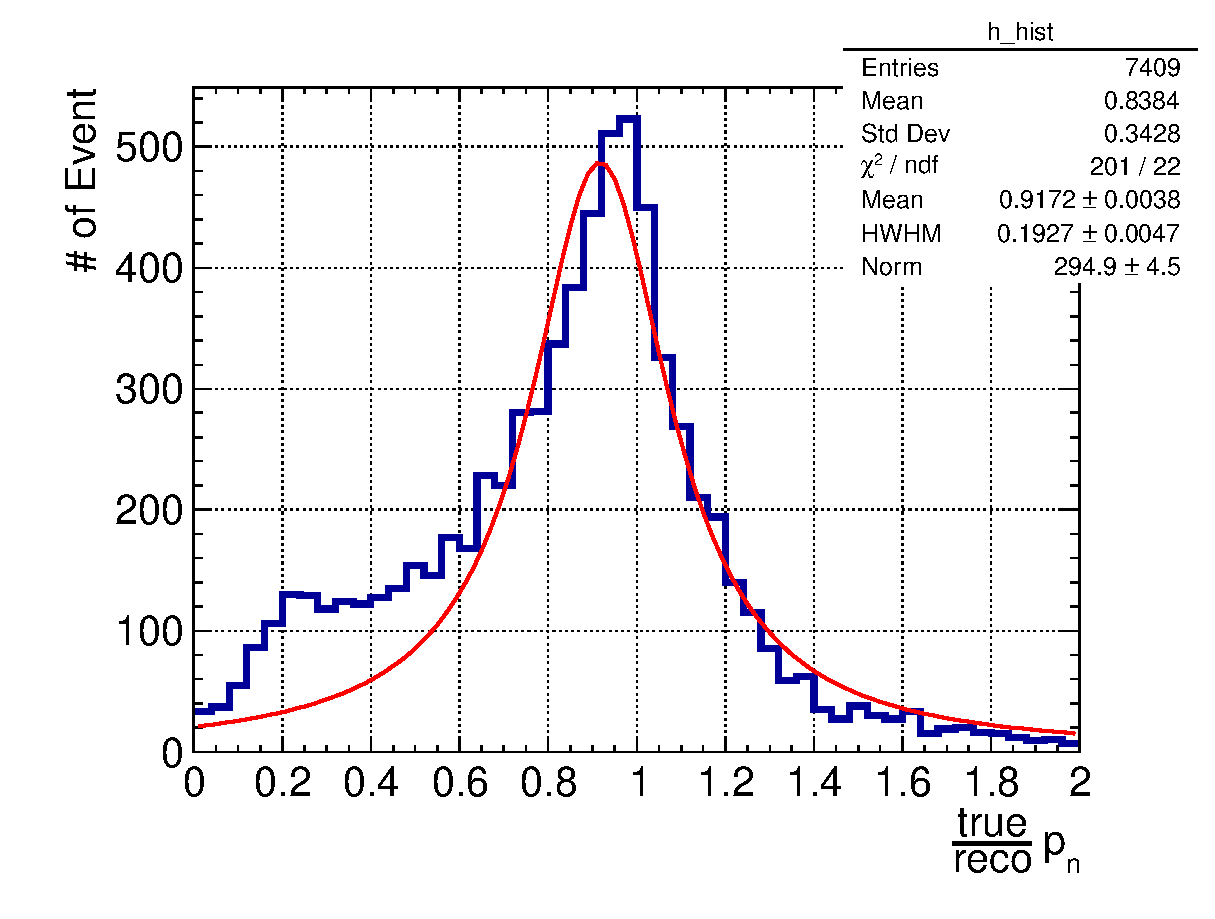
\includegraphics[width=\textwidth]{figures/pn_rat_hist_al13.eps}
                \caption{$\pn$ resolution before ESC selection.}
                \label{fig:pn-res-bfESC}
           \end{subfigure}
           \\
            \begin{subfigure}{0.45\textwidth}
                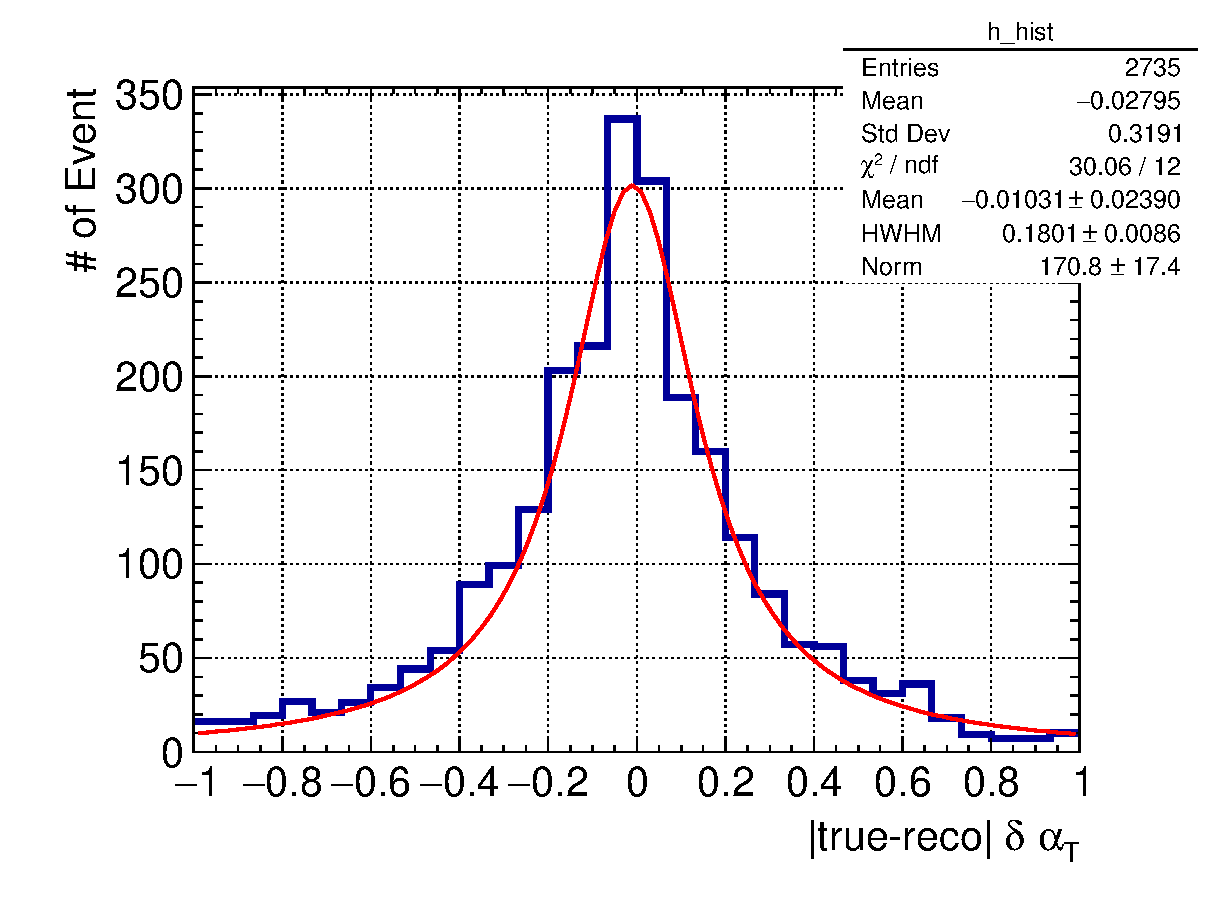
\includegraphics[width=\textwidth]{figures/dalphat_rat_hist_al14.eps}
                \caption{$\dat$ resolution after ESC selection.}
                \label{fig:dat-res-afESC}
           \end{subfigure}
           \begin{subfigure}{0.45\textwidth}
                \includegraphics[width=\textwidth]{figures/pn_rat_hist_al14.eps}
                \caption{$\pn$ resolution after ESC selection.}
                \label{fig:pn-res-afESC}
           \end{subfigure}
           \\
            \begin{subfigure}{0.45\textwidth}
                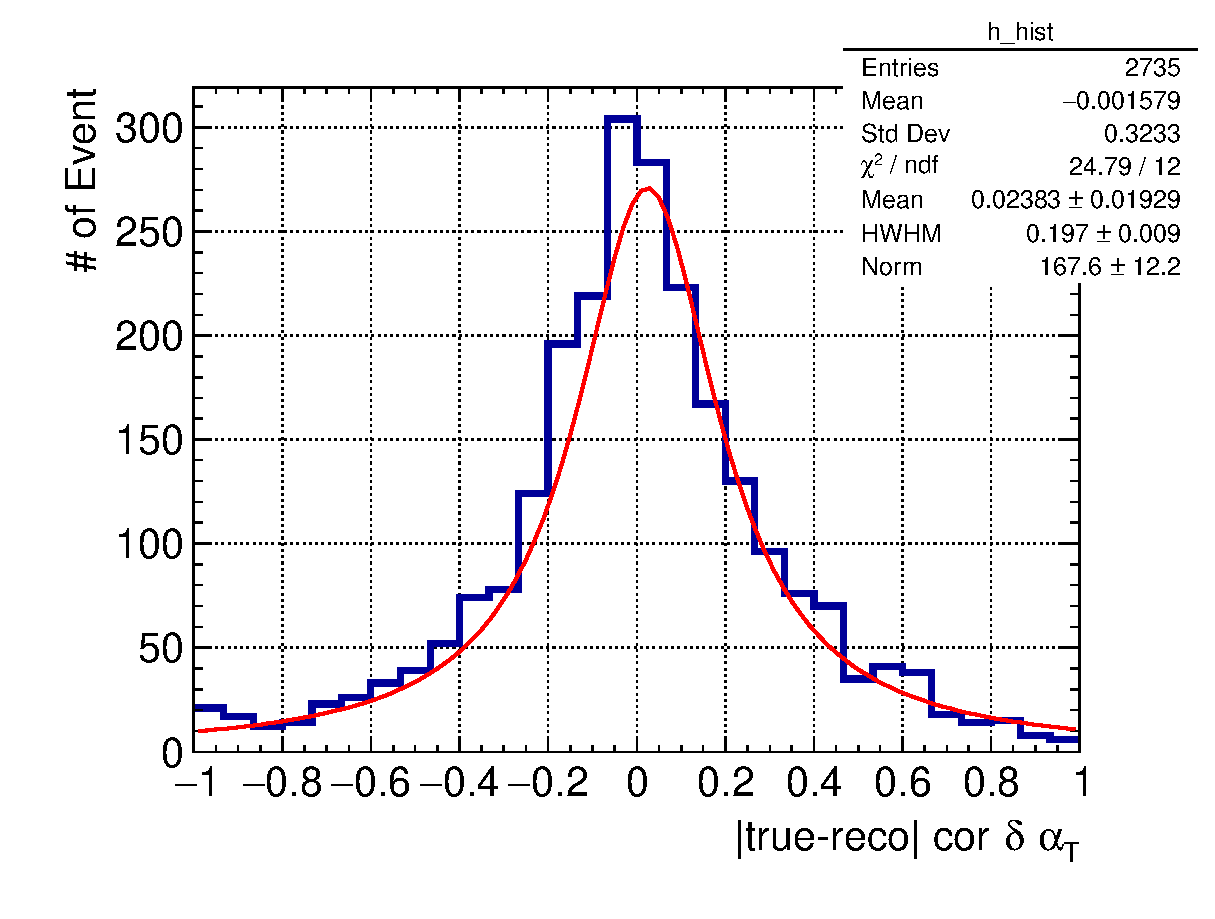
\includegraphics[width=\textwidth]{figures/cor_dalphat_rat_hist_al14.eps}
                \caption{$\dat$ resolution after $\pmut$ correction.}
                \label{fig:0pi-cordat}
           \end{subfigure}
           \begin{subfigure}{0.45\textwidth}
                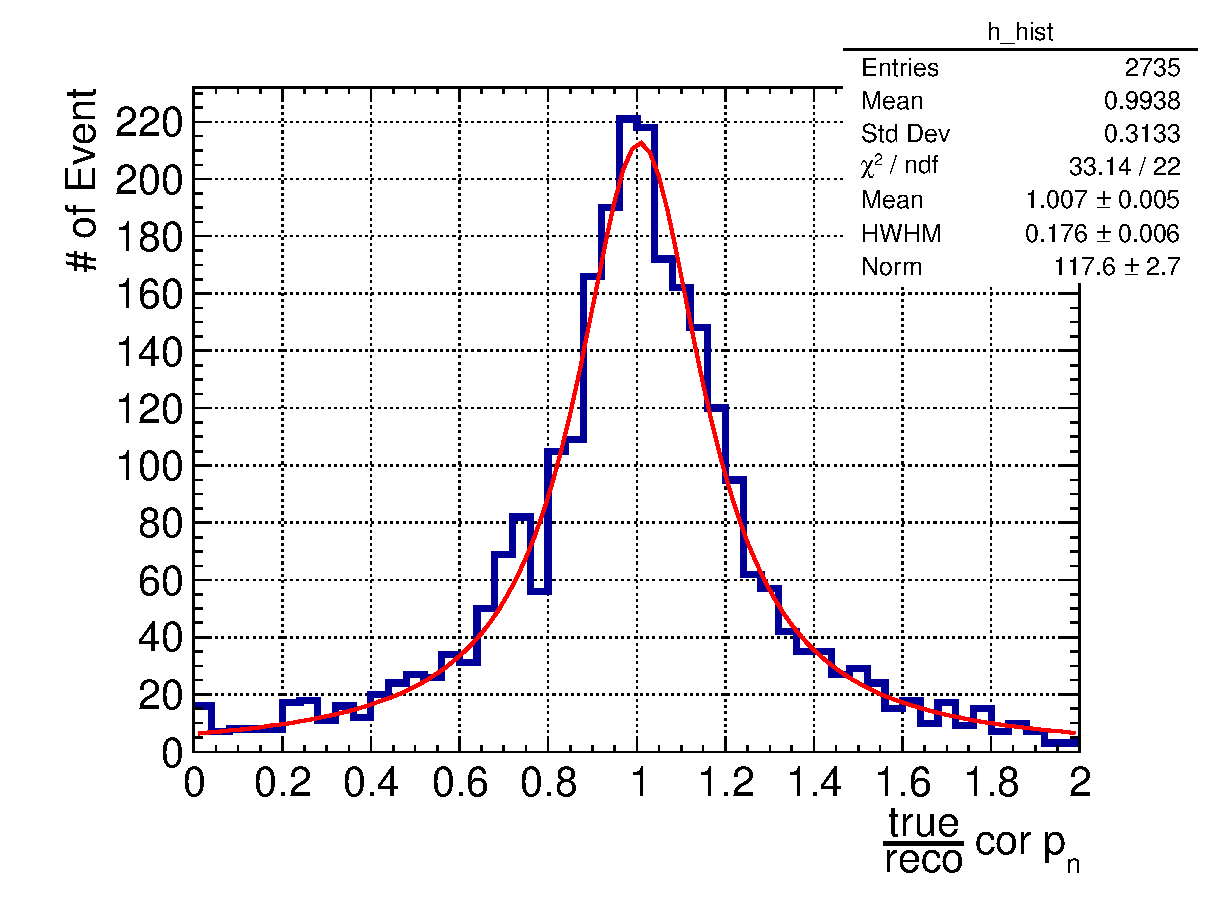
\includegraphics[width=\textwidth]{figures/cor_pn_rat_hist_al14.eps}
                \caption{$\pn$ resolution after $\pmut$ correction.}
                \label{fig:0pi-corpn}
           \end{subfigure}
           \caption{TKI reconstruction results.}
           \label{fig:tki-res-bfafESC}
        \end{figure}

        With the ESC selection, the resolution of $\dat$ and $\pn$ has improved considerably from $0.23$ to $0.18~\textrm{rad}$ and from $19.3\%$ to $14.2\%$ respectively. Moreover, the fitted bias has decreased from $-0.06$ to $-0.01~\textrm{rad}$ and from $1-0.917=0.083$ to $1-0.939=0.061$ for $\dat$ and $\pn$ respectively.  

        As pointed out in Ref.~\cite{Lu:2016mjf}, the ESC selection might lead to a bias in the particle transverse momentum. 
        Such transverse bias would have to be checked after the ESC selection and, if any, corrected for better TKI measurement. 
        The results of the bias check are summarised in Fig.~\ref{fig:0piptbiascheck}. 
        There is no transverse bias for proton as shown in Fig.~\ref{fig:0pi-prpt-bias}, while there is a clear bias in muon $\pt$ for $0.5<\pmut<1.1~(\gevc)$. 
        It is further checked that this bias is not due to a bias in the angle reconstruction, as shown in Fig.~\ref{fig:0pi-mutheta-bias}.
        Thus, a correction is directly applied to $\pmut$ within the specified range, and the corrected $\pmut$ is shown in Fig.~\ref{fig:cormupt}.

       \begin{figure}[!htb]
           \centering
           \begin{subfigure}{0.3\textwidth}
                \includegraphics[width=\textwidth]{figures/pr_pt_vs_pr_pt_bias_hist2d_al14.eps}
                \caption{Proton transverse bias.}
                \label{fig:0pi-prpt-bias}
           \end{subfigure}
           \begin{subfigure}{0.3\textwidth}
                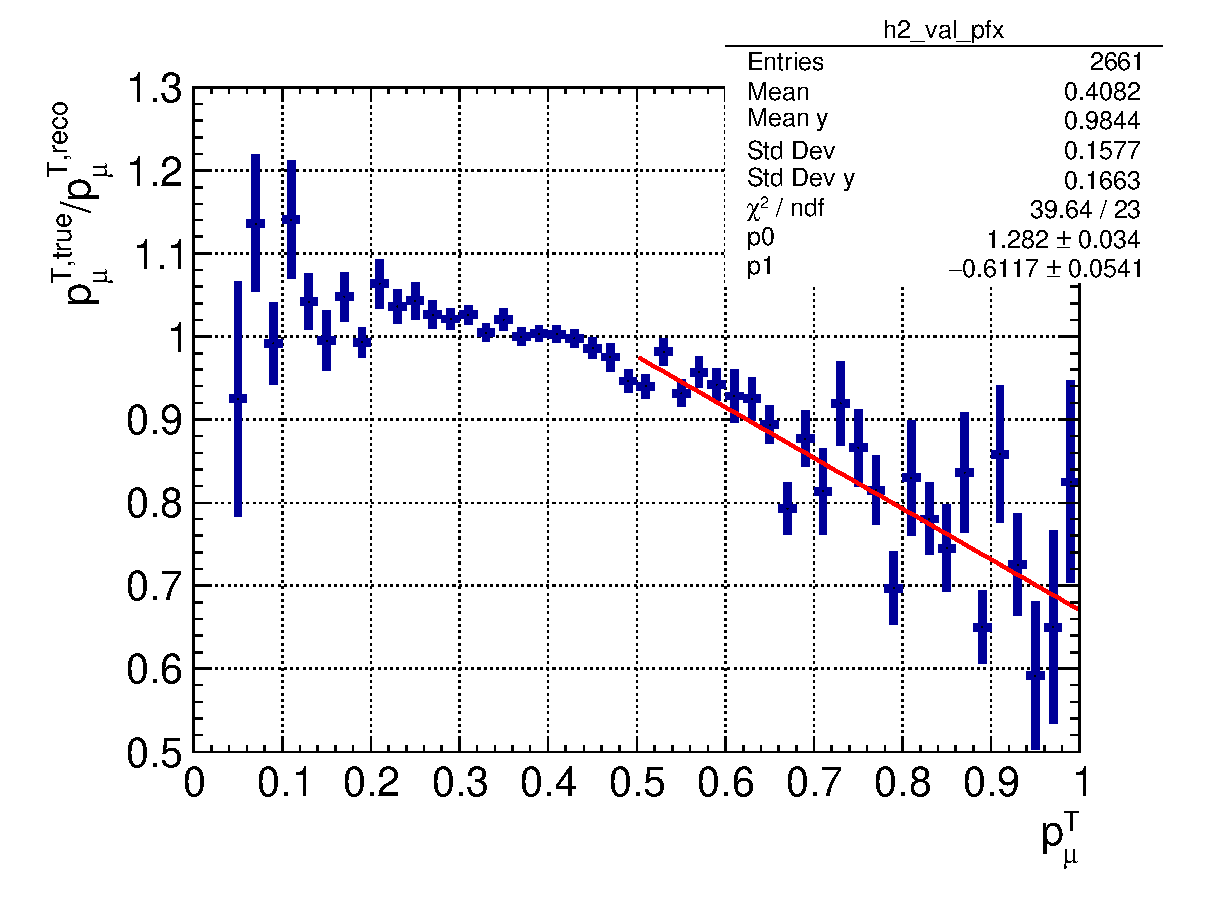
\includegraphics[width=\textwidth]{figures/mu_pt_vs_mu_pt_bias_hist2d_al14.eps}
                \caption{Muon transverse bias.}
                \label{fig:0pi-mupt-bias}
           \end{subfigure}
           \begin{subfigure}{0.3\textwidth}
                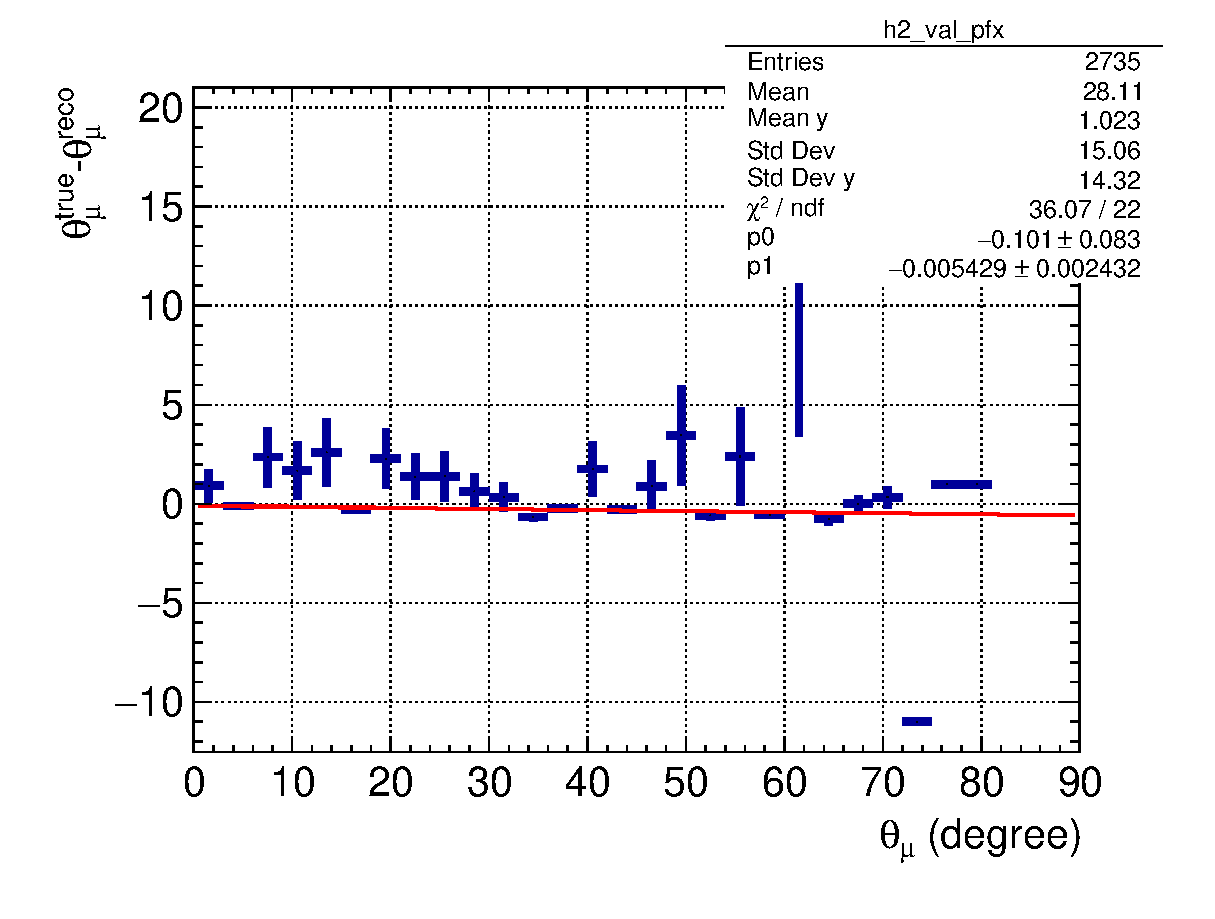
\includegraphics[width=\textwidth]{figures/theta_mu_vs_theta_mu_res_hist2d_al14.eps}
                \caption{Muon theta bias.}
                \label{fig:0pi-mutheta-bias}
           \end{subfigure}
           \caption{Transverse bias check after ESC selection.}
           \label{fig:0piptbiascheck}
        \end{figure}
            
        \begin{figure}[!htb] 	
            \centering 		
            \includegraphics[width=0.35\textwidth]{figures/mu_pt_vs_cor_mu_pt_bias_hist2d_al14.eps}
            \caption{\label{fig:cormupt} Corrected $\pmut$.} 
        \end{figure}

        The impact of the $\pmut$ correction on the TKI variables are shown in Fig.~\ref{fig:0pi-cordat} and Fig.~\ref{fig:0pi-corpn}. The resolutions remain similar, while the bias in $\pn$ has significantly reduced from $6.1\%$ to $0.7\%$.

    \subsection{\label{sec:1pi-tki} TKI in $\numuccopiop$ selection}

    As I have the $\numuccopi$ selection along with the pion trackless reconstruction, it is straightforward to select a $\numuccopiop$ sample by adding an extra step of requiring exactly one SFGD contained proton that passes the ESC selection. 
    The $\pt$ biases are checked for all three particles and no biases are observed. Hence, the final TKI reconstruction results are given in Fig.~\ref{fig:1pi-tki-res}. Both $\dat$ and $\pn$ have minimal fitted bias, $-0.02~\textrm{rad}$ for $\dat$ and about $2\%$ for $\pn$. While the $\dat$ has a slightly worse resolution, $0.24~\textrm{rad}$, than that in $\numucczpiop$, $\pn$ has a better resolution, $12\%$. 
    
   \begin{figure}[!htb] 
       \centering
       \begin{subfigure}{0.45\textwidth}
            \includegraphics[width=\textwidth]{figures/SFGpTPCmu_dalphat_rat_hist_al14.png}
            \caption{$\dat$ resolution.}
            \label{fig:1pi-dat-res}
       \end{subfigure}
       \begin{subfigure}{0.45\textwidth}
            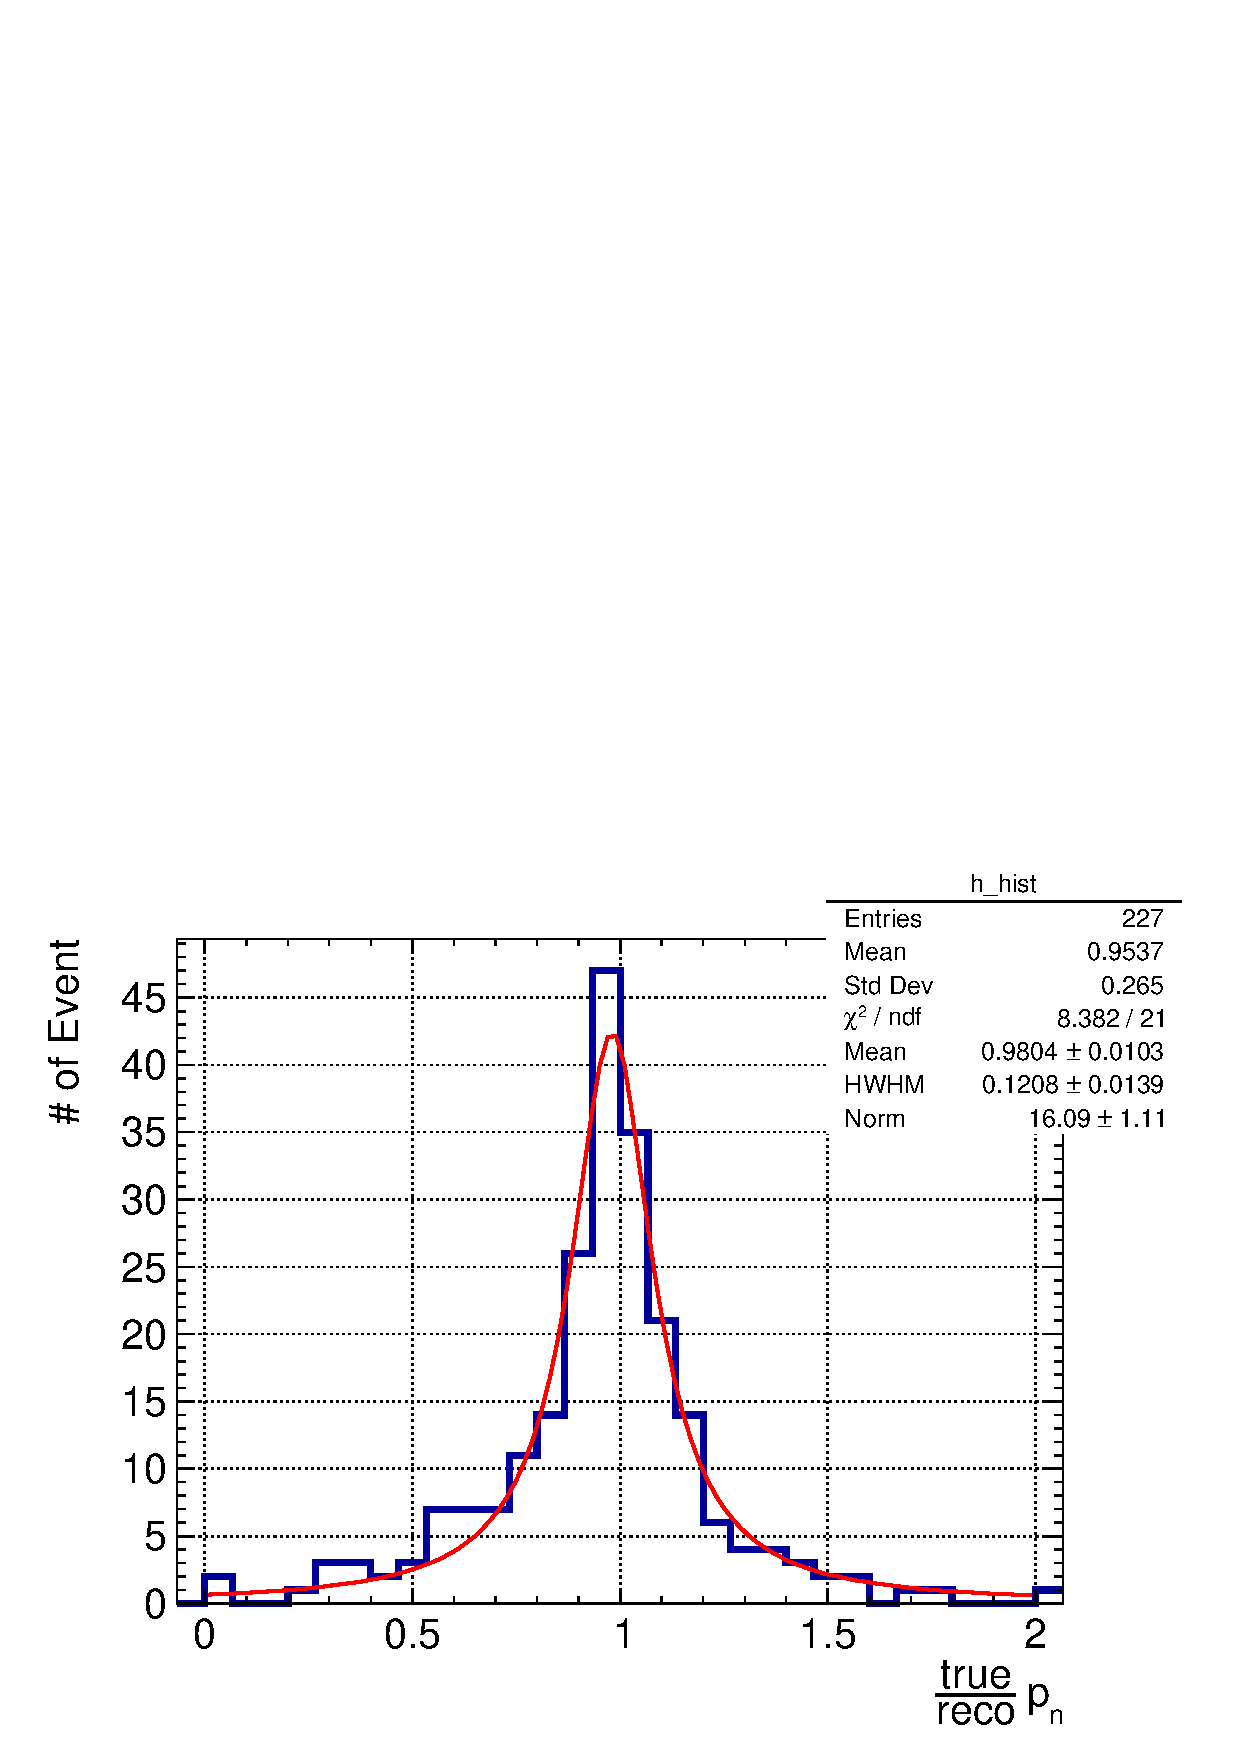
\includegraphics[width=\textwidth]{figures/SFGpTPCmu_pn_rat_hist_al14.png}
            \caption{$\pn$ resolution.}
            \label{fig:1pi-pn-res}
       \end{subfigure}
       \caption{TKI reconstruction results.}
       \label{fig:1pi-tki-res}
    \end{figure}

    In additional to the single transverse variables presented above, the $\numuccopiop$ sample can also be used to measure the double transverse variable, $\dptt$, the net momentum transverse to both the neutrino momentum and the muon momentum,
    Without FSI, $\dptt$ should be $0$. This special property can be exploited to select $\nu$-H events amidst $\nu$-C events as suggested in Ref.~\cite{dpttpaper}. 
    Hence, the main figure of merit for $\dptt$ measurement is the width of its distribution for $\nu$-H events, where the hydrogen events are picked by an additional check on the MC truth information.
    As shown in Fig.~\ref{fig:dptt-hist}, the fitted half width is about $12~\mevc$, which is significantly improved compared to $21~\mevc$, the pre-upgrade ND280 result \cite{dpttpaper}.

    \begin{figure}[!htb] 
        \centering 		
        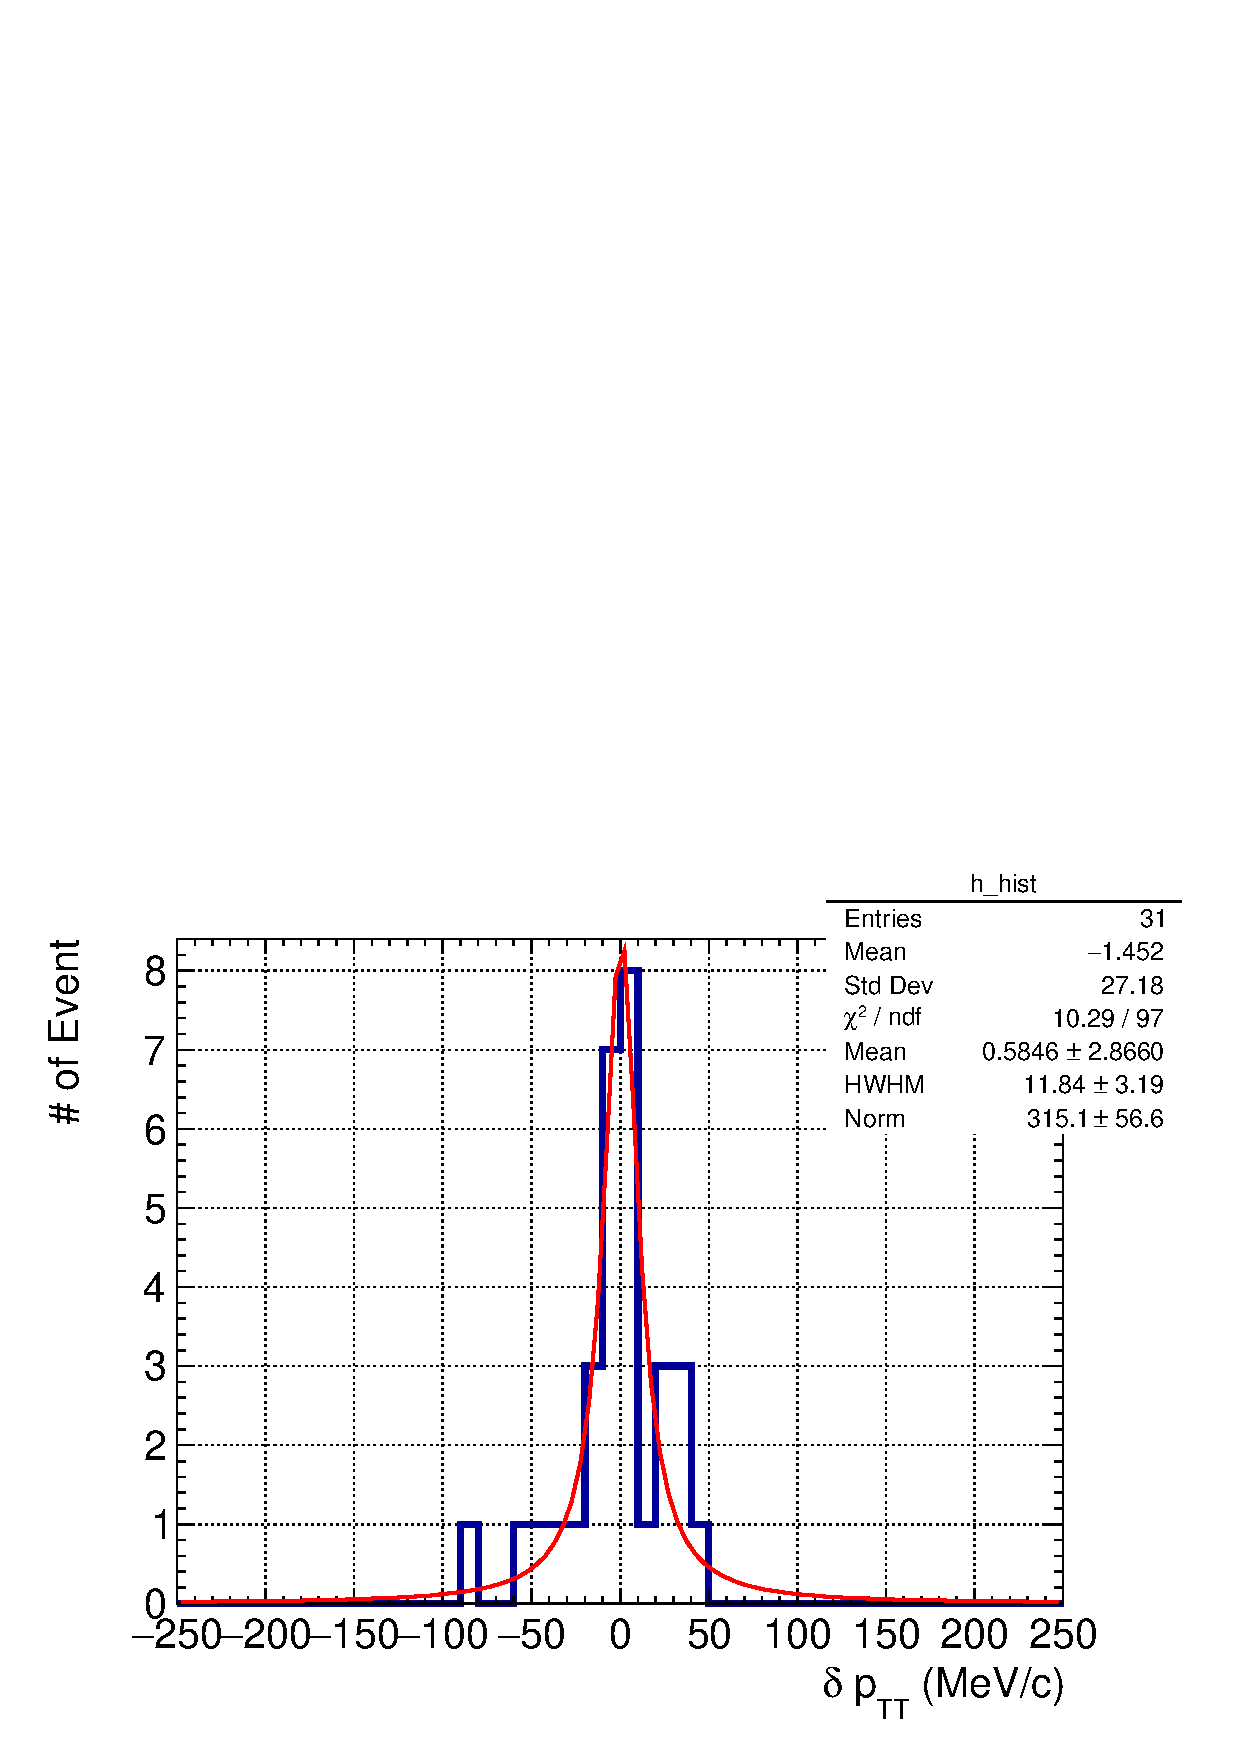
\includegraphics[width=0.35\textwidth]{figures/SFGpTPCmu_dptt_hist_al15_H_bin100_range500_Lfit.png}
        \caption{\label{fig:dptt-hist} $\dptt$ distribution for $\nu$-H events.} 
    \end{figure}


